\documentclass[../Relazione.tex]{subfiles}

\begin{document}
\section{Analisi preliminare}

Questa prima sezione chiarisce di che sito si tratta quello preso in analisi, ne spiega generalmente i suoi contenuti e ne descrive sinteticamente la struttura.

	\subsection{Il nome}
	Nel web, ma anche in generale, la scelta del nome è fondamentale. La media di variazione sull'impatto del pubblico incide dal 10\% al 20\%.\\\\
	Il nome del sito in analisi non rispetta del tutto le regole d'oro: 

	\begin{itemize}
		\item Esso è abbastanza lungo come nome e poteva evidentemente essere ridotto;
		\item È un nome unico che non si confonde con altri siti web;
		\item Possiede un dominio .it e non .com che nella media ha un impatto maggiore del 4,5\% circa;
		\item È facile da memorizzare e da scrivere;
		\item Le parole scelte per la composizione del nome sono già esistenti richiamando tali aspetti;
		\item Il suono della consonante iniziale non è tra quelle consigliate ad ottenere un impatto maggiore.
	\end{itemize}

	Nonostante ciò, il nome del sito fa già molto intendere di che tipologia stiamo parlando, i contenuti che esso tratta e lo sport che evoca.
	È pur sempre vero che lo sport del paintball è molto poco conosciuto ma forse proprio per questo \textbf{viene generata della curiosità} che può spingere l'utente alla visita.
	Inoltre il logo all'interno del sito richiama la maschera protettiva usata in questo sport, che verrà meglio introdotto qui di seguito.\\
	Buona lettura.


\subsection{Il sito}
Descriviamo ora in modo generale il contenuto e la tipologia di questo sito, per poi spiegare più nel dettaglio l'offerta che viene posta al cliente/utente in visita.
	\subsubsection{Overview generale}
	\paint\ è il sito dell'associazione sportiva denominata \textbf{NordEst Paintball}, che presenta le offerte e gli eventi legati alle partite di paintball che si possono fare all'interno della loro sede e quindi dei loro campi da giuoco appositamente creati.
	Il sito preso in esame contiene una galleria di immagini realmente scattate nel luogo durante alcune partite, una mappa per raggiungere la struttura oltre che ovviamente una sezione per il listino dei prezzi per tipologia e tempo di gioco.
\newpage
	\subsubsection{Il paintball}
	\textbf{Ma che sport è il paintball? E come si gioca?}...scopriamolo assieme poichè è davvero molto interessante anche se poco conosciuto...\\
	Il paintball ha come scopo, nei casi più comuni, di rubare la bandiera in base avversaria riportandola in base propria tramite l'eliminazione della squadra avversaria.
	I partecipanti tentano di colpirsi con delle palline di gelatina riempite di vernice colorata, sparate mediante appositi strumenti ad aria compressa chiamati marker (marcatori). Data la velocità d'impatto (al massimo 300 piedi al secondo, 328 km/h per le competizioni internazionali), la capsula della paintball si rompe al contatto con l'obiettivo, rilasciando il contenuto sugli abiti dell'avversario o su qualsiasi altro oggetto col quale impatti. Una volta contrassegnato da una "paintball", un giocatore è eliminato dal game (o sospeso per un breve tempo, 60 secondi di solito). Questo sport viene regolarmente praticato anche a livello agonistico in competizioni, tornei e campionati ufficiali in tutto il mondo. Le paintball per legge devono essere totalmente biodegradabili, atossiche ed ecocompatibili.
	Per approfondimenti seguire il link della fonte qui di seguito.
	[ fonte: \href{https://it.wikipedia.org/wiki/Paintball}{Wikipedia} ]\vspace{1cm}

	\begin{figure}[!h]
		\centering
			\begin{minipage}[c]{.50\textwidth}
			  \centering\setlength{\captionmargin}{0pt}%
			  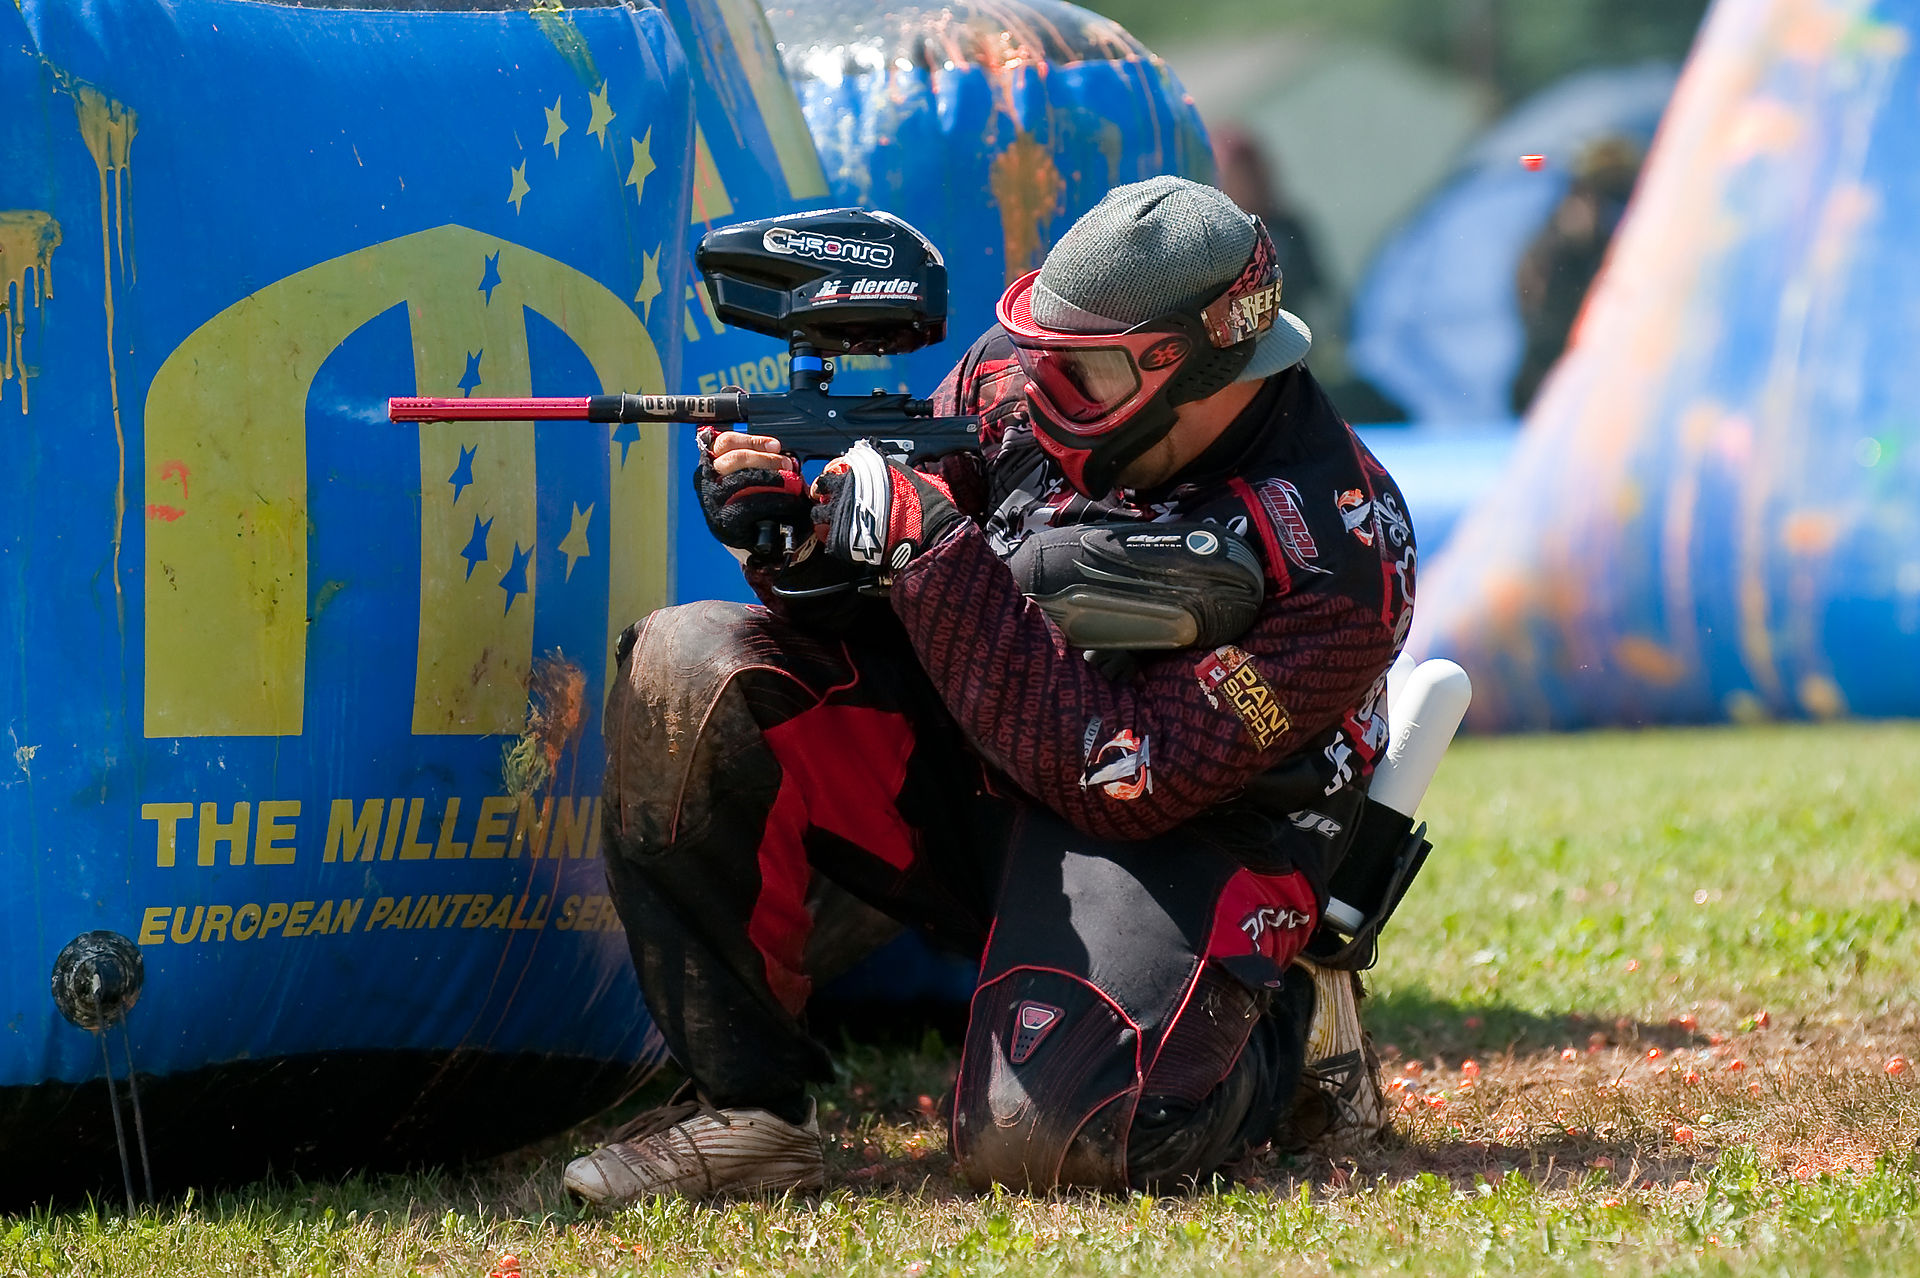
\includegraphics[scale=0.42]{img/sport/player1.jpg}
			  \caption{Giocatore di paintball}
			\end{minipage}%
			\hspace{10mm}%
			\begin{minipage}[c]{.40\textwidth}
			  \centering\setlength{\captionmargin}{0pt}%
			  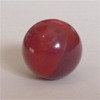
\includegraphics[width=.40\textwidth]{img/sport/paint.png}
			  \caption{Capsula di paintball}
			\end{minipage}
		\label{fig:minipage2}
	\end{figure}

\newpage	
	\subsection{La struttura}
		Il sito presenta la seguente struttura gerarchica di pagine:
		\begin{itemize}
			\item \textbf{Homepage}: Cerca di colpire ed accogliere gli utenti descrivendo un po il luogo di gioco anche con qualche immagine;
			\item \textbf{Eventi}: Descrive i 4 possibili eventi legati alla struttura ed ai campi;
			\item \textbf{Gallery}: Presenta una slideshow di fotografie reali durante alcuni game;
			\item \textbf{Dove siamo}: Descrizione di come arrivare alla struttura ed inserimento di una mappa Google con segnaposto all'indirizzo;
			\item \textbf{Listino}: Presentazione dei vari pacchetti disponibili ai clienti in termini di tempo, accesso ai vari campi, dotazione e prezzi a persona;
			\item \textbf{Contatti}: Informazioni di contatto e form per la richiesta di ulteriori chiarimenti o preventivi.
		\end{itemize}
		
		La gerarchia del sito è molto semplice, difatti non presenta contenuti di secondo livello ma espande tutte le informazioni necessarie nelle sezioni sopra descritte, tutte chiaramente visibili nel menù orizzontale.
		Per la tipologia commerciale e lo scopo del sito (quello di incuriosire ed invogliare più utenti possibili a giocare recandosi nel posto) questa semplicità si trasforma in chiarezza diventando quindi, a mio parere, un fattore positivo.
		Di seguito anche un riassunto del numero dei link che interessano completamente il sito, ottenuto in automatico tramite il servizio a questo \href{http://smallseotools.com/website-links-count-checker/}{link}.

		\begin{figure}[!h]
			\centering
			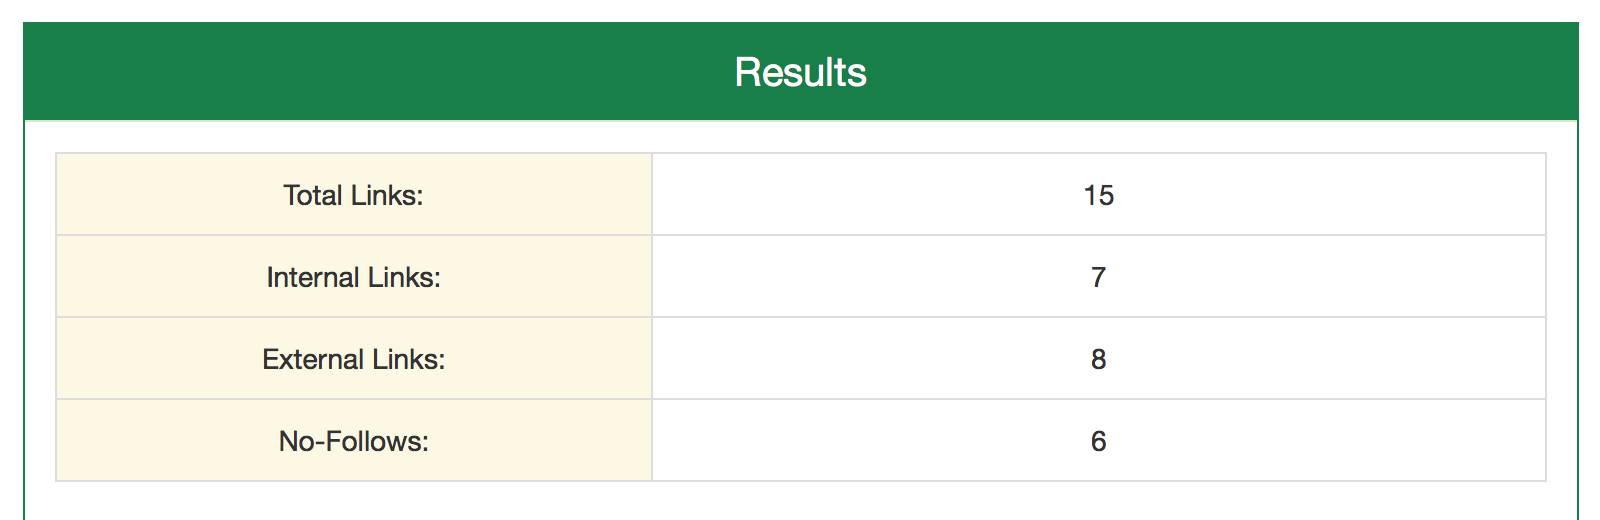
\includegraphics[width=0.95\textwidth]{img/sito/LinksReport.png}
			\caption{Links report dell'intero sito}
			\label{fig:links}
		\end{figure}
\end{document}
		